\section{问题四：女胎异常判定模型的建立}
为对女胎染色体异常情况进行判定，本文建立并评估了多种机器学习模型。数据集中正常与异常样本比例约为9比1，属于类别不平衡问题。研究的核心在于提升模型对少数异常样本的识别能力，即召回率，以满足临床筛-查的应用需求。本章阐述了数据准备，模型训练，性能评估与模型解释的完整过程。

\subsection{模型准备与评估方法}

\subsubsection{数据划分与不平衡处理}
为建立公平的训练与评估环境，我们首先将所有经过预处理的女胎数据，依据7比3的比例执行分层抽样，分别划分为训练集与测试集。分层操作确保了两个数据子集中的异常样本比例与原始数据集保持一致。

为应对数据类别不平衡的问题，我们仅对训练集应用了合成少数类过采样技术SMOTE。该技术通过在少数类样本附近合成新的样本实例来增加其数量。我们将训练数据中异常样本与正常样本的比例由约1比9提升至1比2。这种采样比例的目的是在增强模型对少数类别学习能力的同时，避免因引入过多人工样本而可能出现的过拟合现象。测试集则维持其原始数据分布。

\subsubsection{候选模型介绍}
为完成对女胎染色体异常的判定，本文选取了三种不同的分类算法进行训练与比较。这些算法分别是逻辑回归、决策树与XGBoost，它们在模型结构和学习方式上各有特点，能够从不同层面分析数据。

逻辑回归是一种用于处理二元分类问题的统计方法。该模型通过一个特定的函数，即逻辑斯谛函数，将自变量的线性组合映射到0至1的区间内，所得到的数值可以被解释为某个事件发生的概率。对于给定的输入特征向量$X$，其属于正类的概率$p(X)$的计算方式为
\begin{equation}
p(X) = \frac{1}{1 + e^{-(\beta_0 + \sum_{i=1}^{n} \beta_i X_i)}}
\end{equation}
在此式中，$\beta_0$是截距项，$\beta_i$是第$i$个特征$X_i$对应的模型系数。这些系数是通过对训练数据的学习过程估计得出的，通常采用最大似然估计法进行求解。当模型输出的概率值大于预设的阈值，一般为0.5时，样本被判定为正类，反之则为负类。


决策树是一种基于树状结构进行决策的非参数学习算法。该模型通过从数据中学习一系列分层的是非问题来对样本进行分类。整个模型的结构形似一棵倒置的树，其中每个内部节点代表对一个特征属性的测试，从该节点引出的每个分支代表测试的一个可能结果，而每个叶节点则代表一个最终的类别标签。决策树的生成是一个递归过程，在每一步，算法会选择一个最优的特征来划分数据集，划分的准则通常是使得划分后数据的纯度最高，例如使用信息增益或基尼不纯度作为度量。这个划分过程会持续进行，直到子集中的所有样本都属于同一类别，或者达到其他预设的停止条件。

XGBoost是梯度提升框架下的一种算法实现。它属于集成学习方法，通过迭代式地生成一系列弱学习器，通常是决策树，并将它们组合起来形成一个表现更好的学习模型。该算法以序列化的方式构建模型，在每一轮迭代中，一个新的决策树被训练出来，其目标是修正前面所有树组成的集成模型所犯的错误。具体而言，新的树拟合的是损失函数关于前一轮模型预测结果的负梯度，即残差。第$t$轮迭代后，对样本$x_i$的预测值$\hat{y}_i^{(t)}$由前一轮的预测值与当前轮新加入的树模型$f_t(x_i)$共同构成
\begin{equation}
\hat{y}_i^{(t)} = \hat{y}_i^{(t-1)} + f_t(x_i)
\end{equation}
最终的预测结果是所有轮次生成的树模型输出值的总和。该方法在损失函数中加入了正则化项，用以控制模型的复杂度，从而防止过拟合。

\subsubsection{模型优化与评估指标}
为使各模型达到其最优状态，本文采用网格搜索与交叉验证相结合的方法进行超参数调优。网格搜索能够系统性地遍历预先设定的参数组合，从而避免了人工试错的随意性。与交叉验证方法结合使用，可以在不同数据子集上反复评估每一种参数组合的性能，其结果能够比单次划分训练集和验证集提供更稳健的模型泛化能力度量，减少了因特定数据划分而引起的偶然性。

具体实施5折分层交叉验证，其优势在于分层抽样保证了每一个折叠中的类别比例都与原始训练集保持一致。在处理类别数量不均衡的数据时，此种方法可确保少数类的样本在每次训练和验证中都得到体现，从而获得更可靠的性能估计。将此过程应用于经过SMOTE技术处理后的训练数据，其目的是在不影响测试集真实分布的前提下，缓解模型训练时对多数类的偏向。

将网格搜索的优化评分指标设定为召回率，是直接响应本任务的应用需求。在异常检测的场景下，漏掉一个异常样本的代价远高于将正常样本误判。召回率这一指标直接衡量模型找出所有真实异常样本的能力。因此，以召回率为优化目标，能够使超参数的选择过程导向于构建一个尽可能减少漏诊的模型，使模型的功能与实际应用目标保持一致。



\subsection{模型性能比较分析}
在模型调优完成后，我们在原始的、未曾见过的测试集上，通过多维度指标对三个模型进行评估，并以此为依据选择最终模型。评估的首要指标是异常类别的召回率，该指标直接度量模型避免漏诊的能力。当召回率相近时，则依次比较F1分数、AUC值以及精确率。

\begin{figure}[h!]
\centering
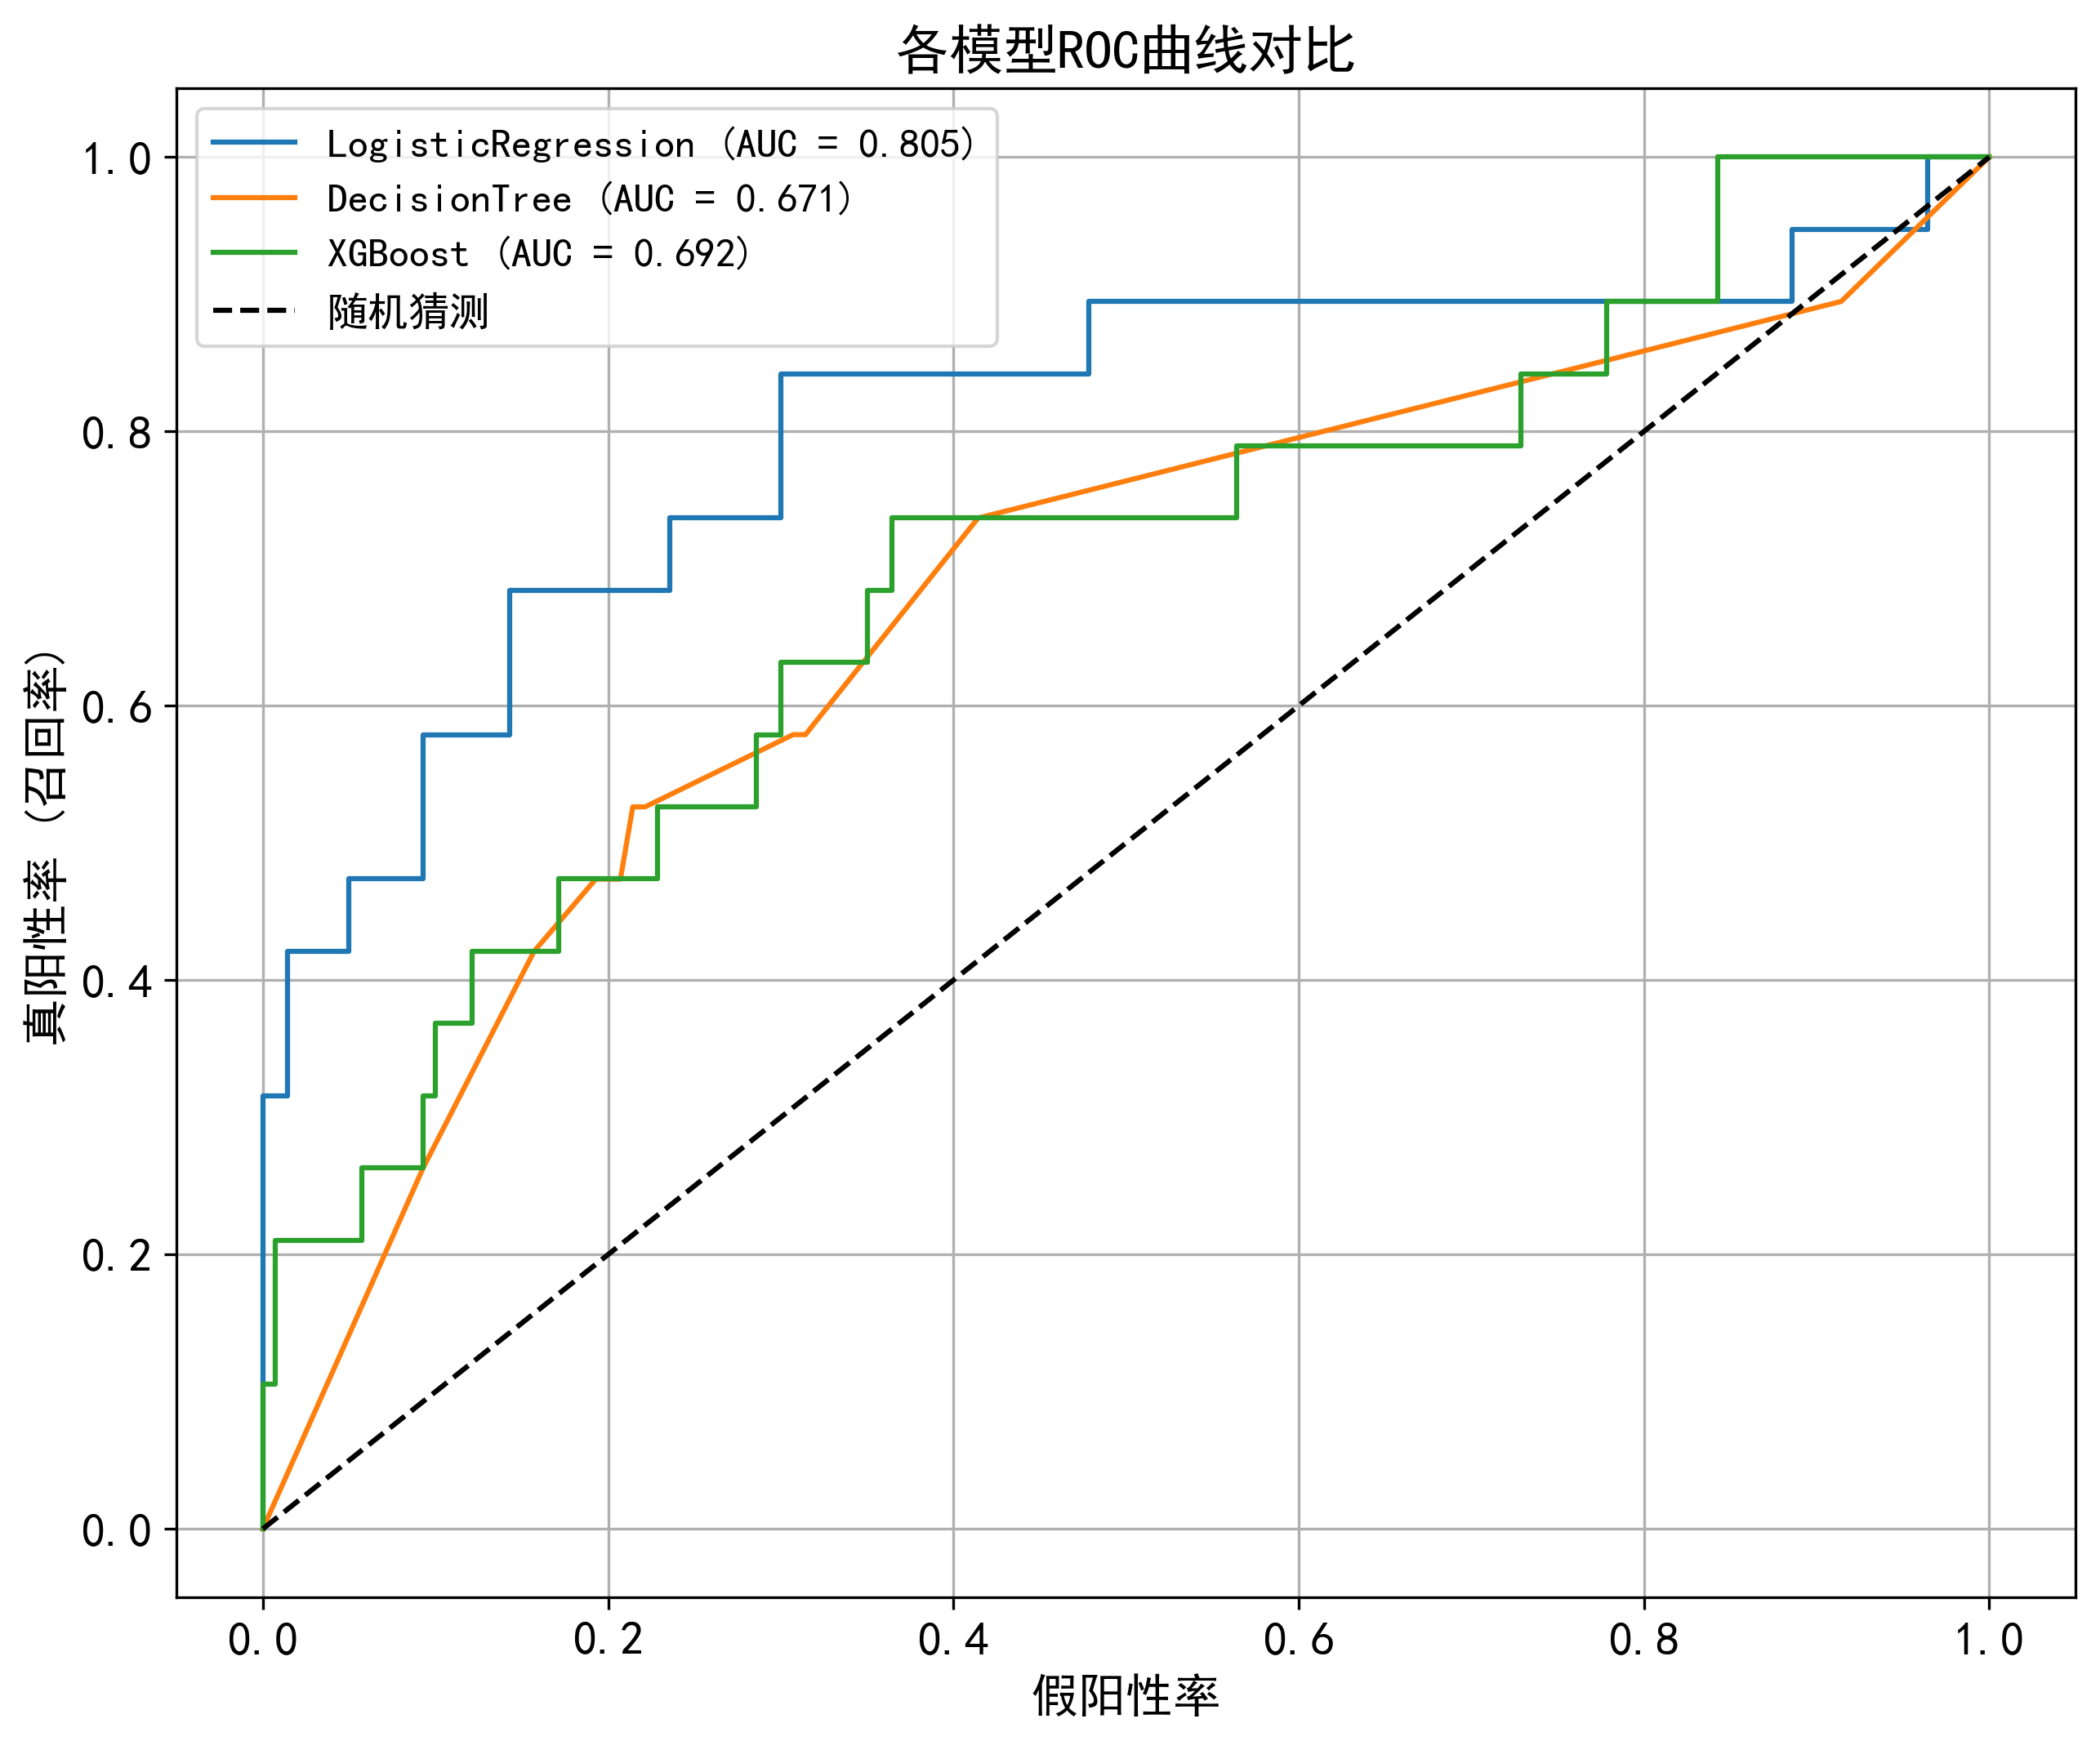
\includegraphics[width=0.8\textwidth]{figs/6问题四/图10_模型ROC曲线对比.png}
\caption{模型ROC曲线对比}
\label{fig:roc_curve}
\end{figure}

\cref{fig:roc_curve}展示了三个模型在不同阈值设定下区分正常与异常样本的整体能力。图中曲线越靠近左上角，其下方的面积即AUC值越大，说明模型的诊断价值越高。逻辑回归模型的ROC曲线，其AUC值为0.805，优于决策树的0.671和XGBoost的0.692。逻辑回归的曲线包裹了更大的面积，表明其在所有阈值下的判别能力相对更优。

\begin{figure}[h!]
\centering
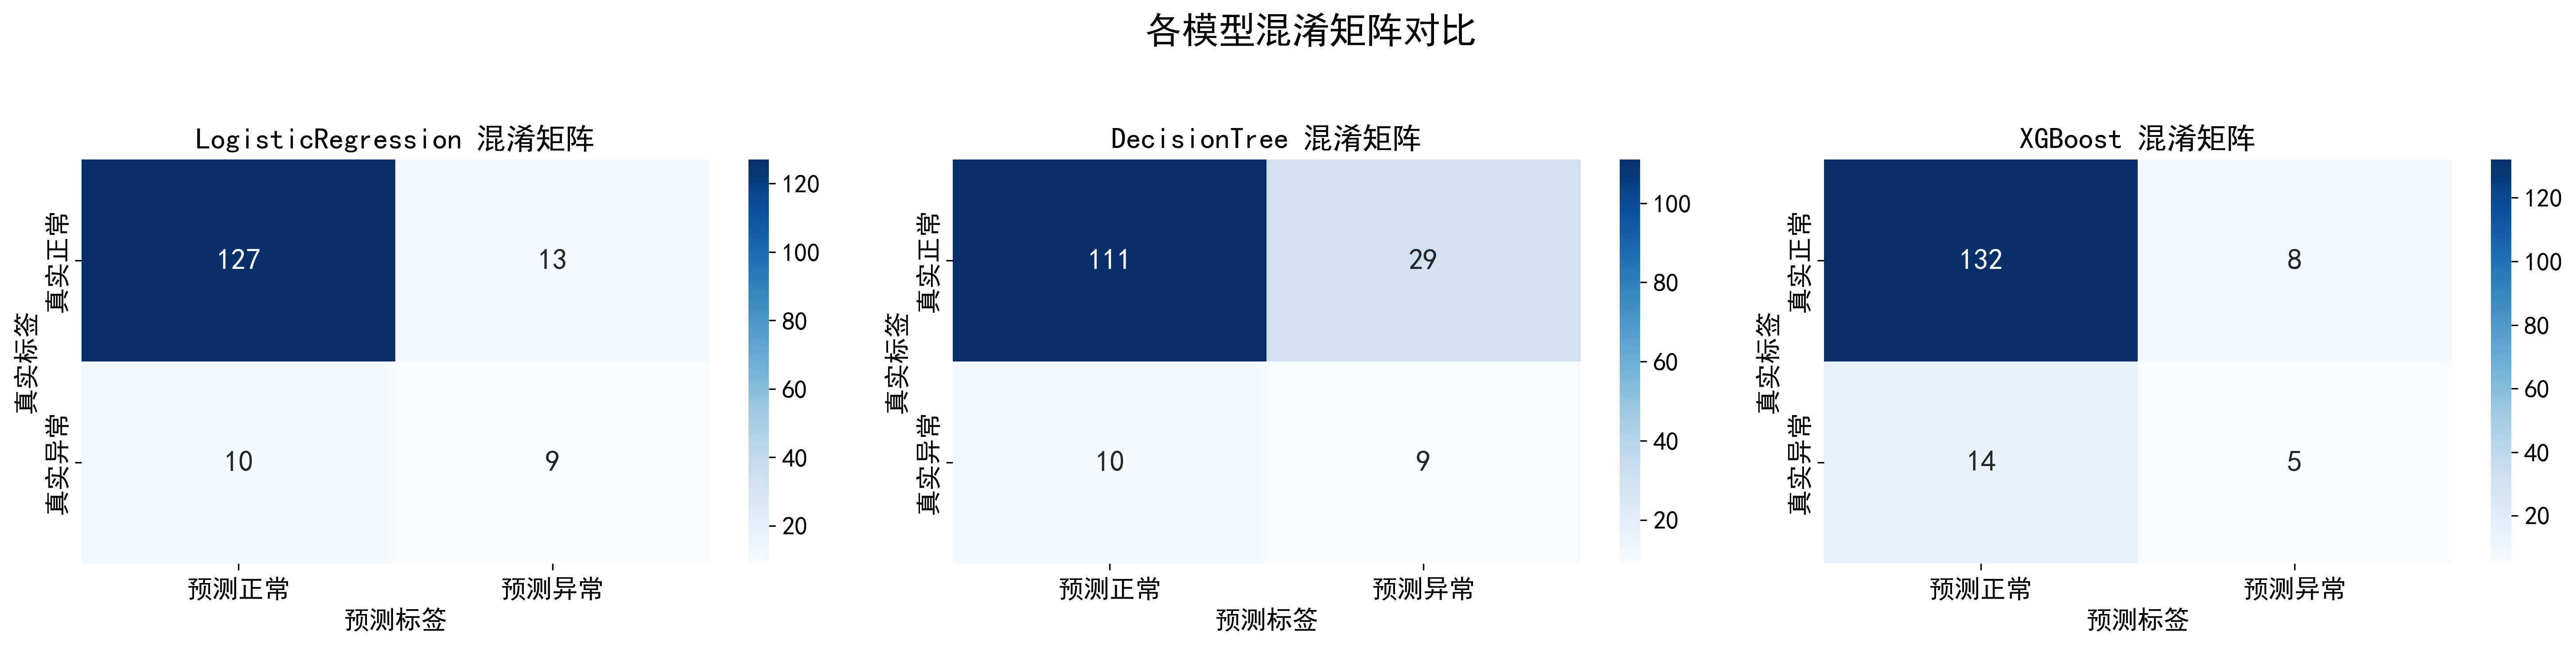
\includegraphics[width=1\textwidth]{figs/6问题四/图11_模型混淆矩阵对比.png}
\caption{模型混淆矩阵对比}
\label{fig:confusion_matrix_comp}
\end{figure}


\cref{fig:confusion_matrix_comp}展示了各模型在测试集上的具体预测分布。测试集中共包含19例真实的异常样本。逻辑回归与决策树均成功识别出其中的9例，对应10例漏诊，两者的召回率均为47.4百分比。XGBoost模型仅识别出5例，漏诊14例。在误诊方面，逻辑回归将13例正常样本错误判断为异常，而决策树的误诊数量为28例。此结果表明，在查全能力相同的情况下，逻辑回归的查准能力更优。

\begin{table}[h!]
\centering
\caption{各候选模型在测试集上的性能指标对比}
\label{tab:model_performance}
\begin{tabular}{lcccc}
\toprule
模型 & 精确率 & 召回率 & F1分数 & AUC \\
\midrule
LogisticRegression & 0.409 & 0.474 & 0.439 & 0.805 \\
DecisionTree & 0.237 & 0.474 & 0.316 & 0.671 \\
XGBoost & 0.385 & 0.263 & 0.313 & 0.692 \\
\bottomrule
\end{tabular}
\end{table}

\cref{tab:model_performance}对各模型针对异常样本的各项性能指标进行了量化总结。根据此表，逻辑回归与决策树在首要指标召回率上均达到0.474，并列最高。为作出最终选择，需要比较次要指标。逻辑回归的F1分数为0.439，高于决策树的0.316，这表明逻辑回归在精确率与召回率之间取得了更好的平衡。同时，逻辑回归的精确率为0.409，同样高于决策树的0.237，并且其AUC值0.805也是三者中最高的。因此，基于各项关键评估维度的数值，逻辑回归模型被选定为最终的判定模型。



\subsection{最优模型解释性分析}
为解释逻辑回归模型判定女胎异常的具体依据，本文采用SHAP方法进行模型解释。SHAP的全称为SHapley Additive exPlanations，该方法建立在合作博弈论中的夏普利值理论之上，为机器学习模型的预测结果提供解释。其核心思想是将数据样本的每一个特征视为参与一场合作的成员，而最终回报即为模型的预测输出。对于单个预测样本，SHAP值能够计算出每个特征在所有可能的特征组合中对预测结果的平均边际贡献，从而将模型的预测值公平地分配给各个特征。一个可解释的模型$g(z')$可以用所有特征的SHAP值$\phi_j$线性相加来表示
\begin{equation}
g(z') = \phi_0 + \sum_{j=1}^{M} \phi_j z'_j
\end{equation}
在此式中，$\phi_0$代表了数据集中所有样本预测值的平均，也称为基准值。$\phi_j$即为第$j$个特征的SHAP值，它量化了该特征将模型预测结果从基准值推向最终预测值的贡献大小和方向。正值的SHAP值表示该特征促使模型预测结果向正类别移动，负值则代表其作用相反。

\begin{figure}[h!]
    \centering
    \begin{minipage}[t]{0.48\textwidth}
        \centering
        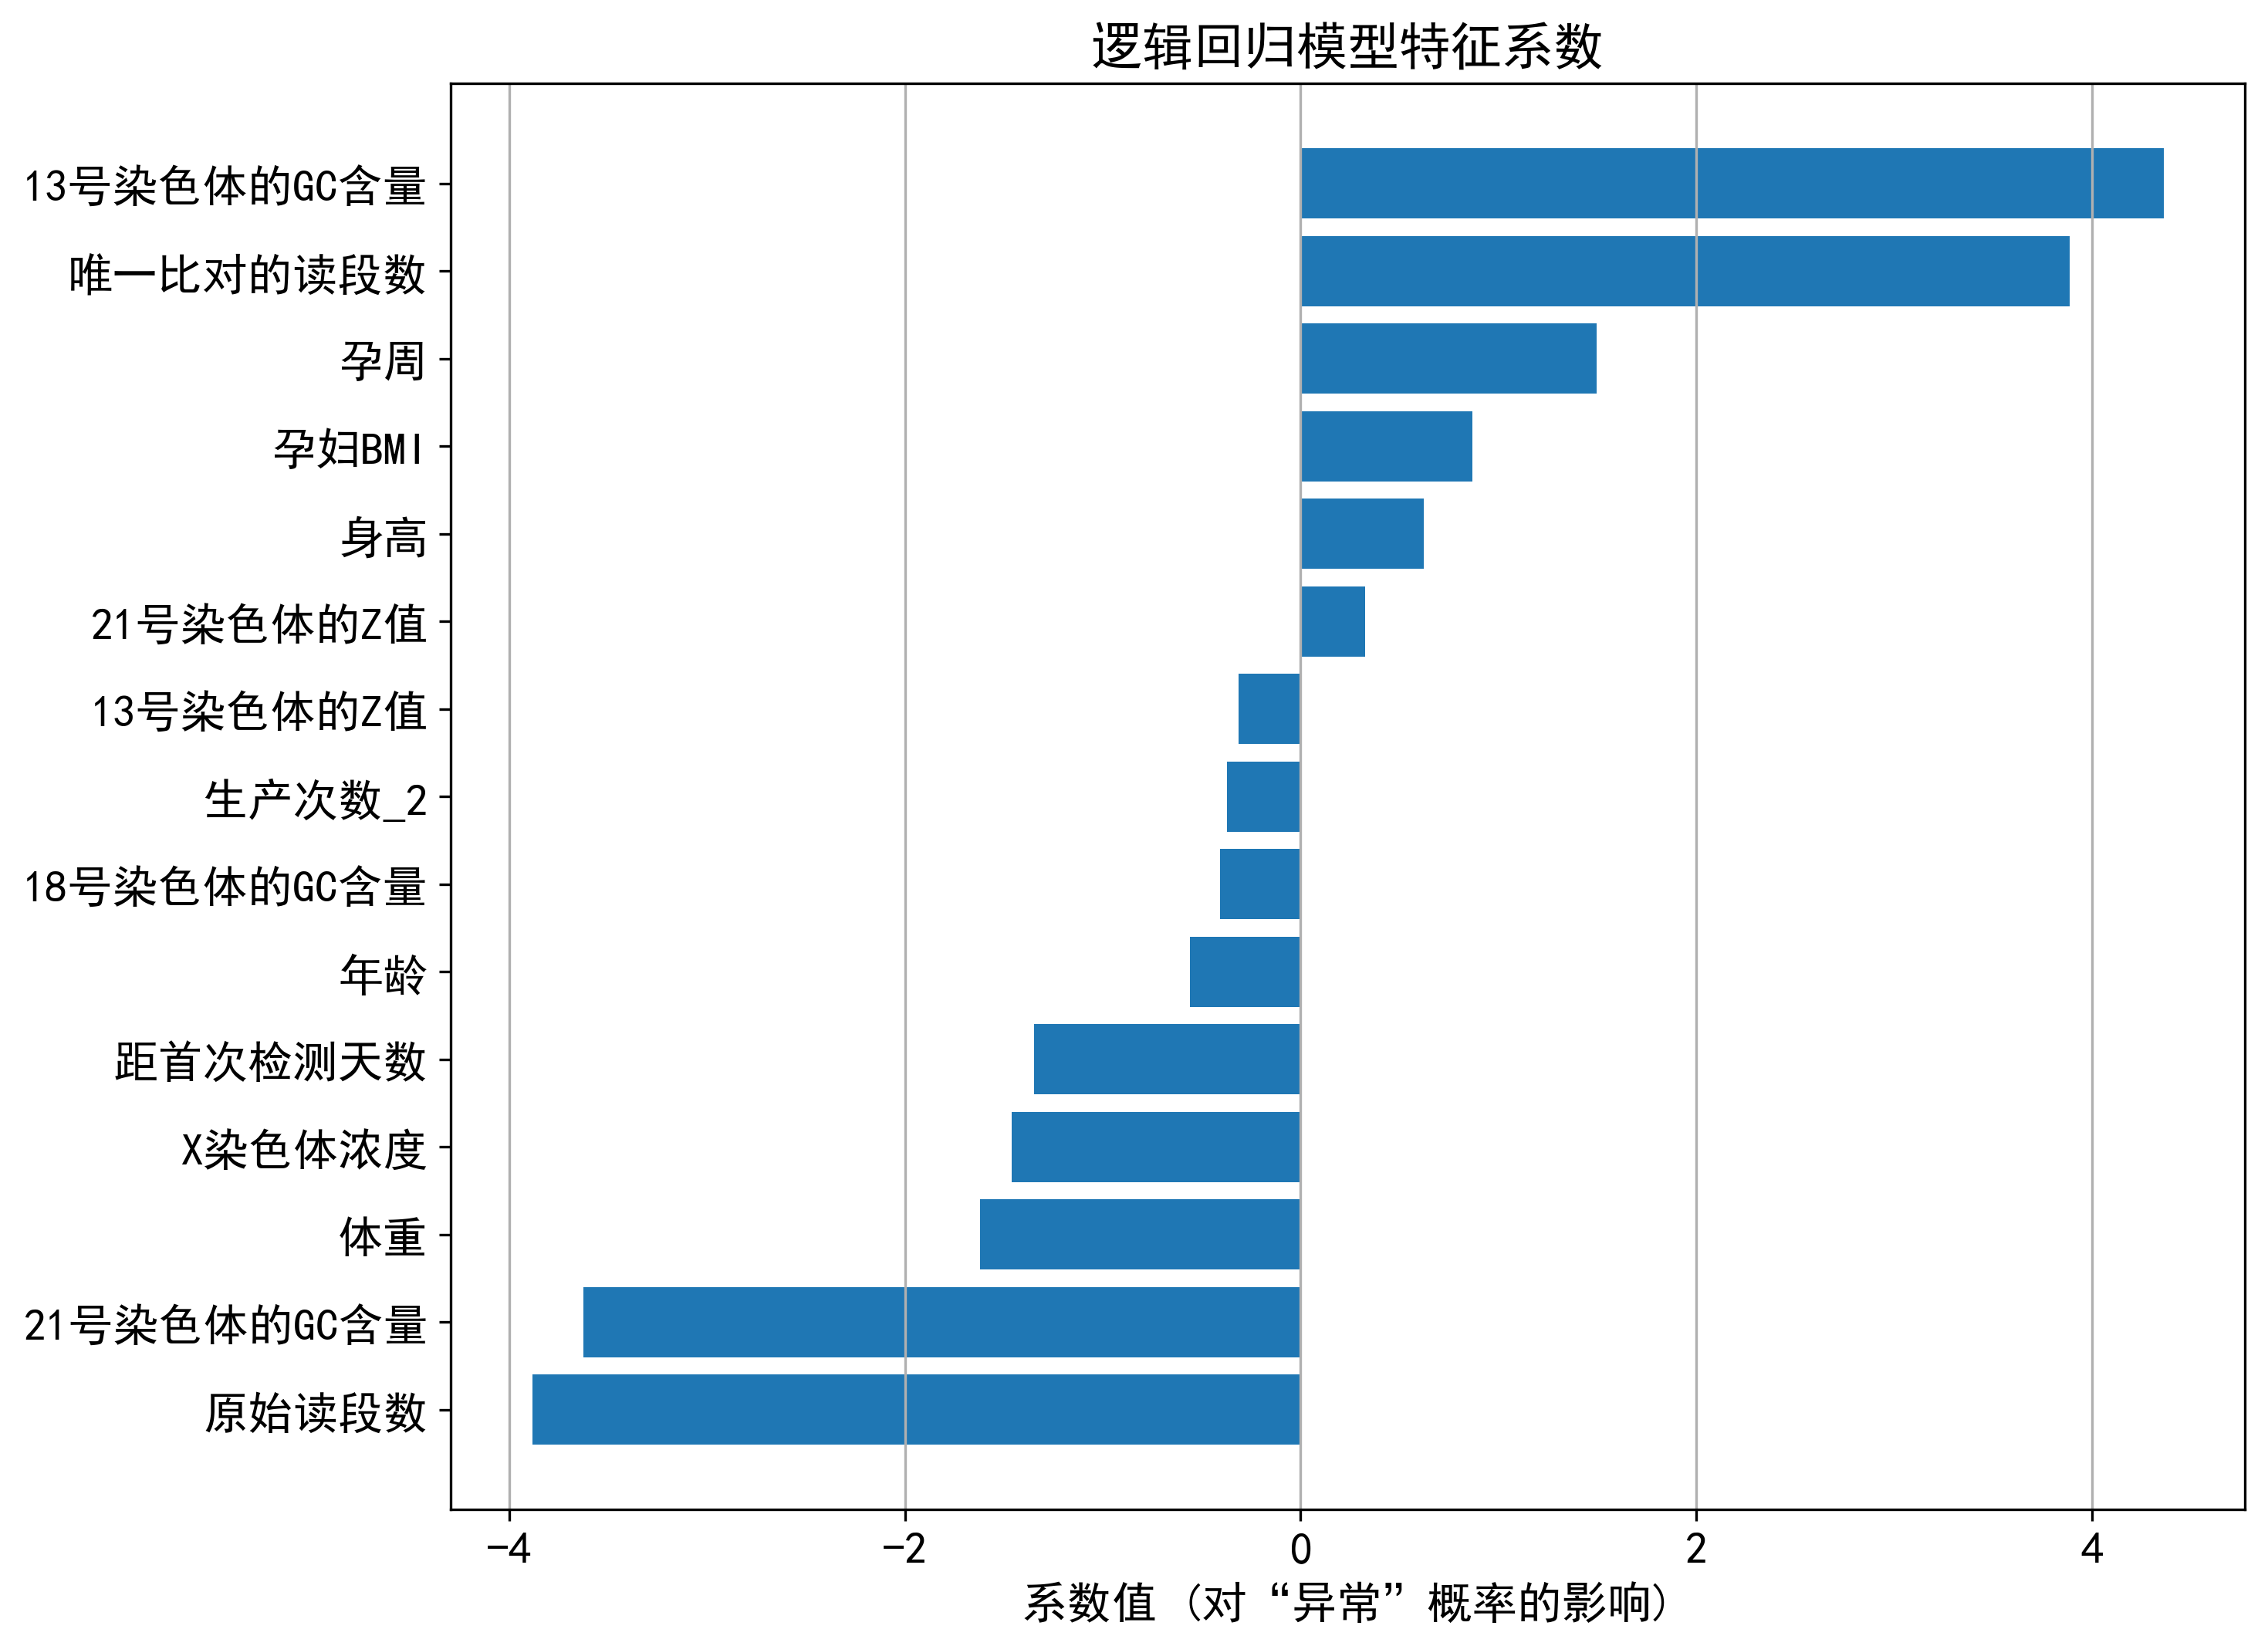
\includegraphics[width=\textwidth]{figs/6问题四/图12_逻辑回归特征重要性.png}
        \caption{逻辑回归模型特征重要性排序}
        \label{fig:feature_importance}
    \end{minipage}
    \hfill
    \begin{minipage}[t]{0.48\textwidth}
        \centering
        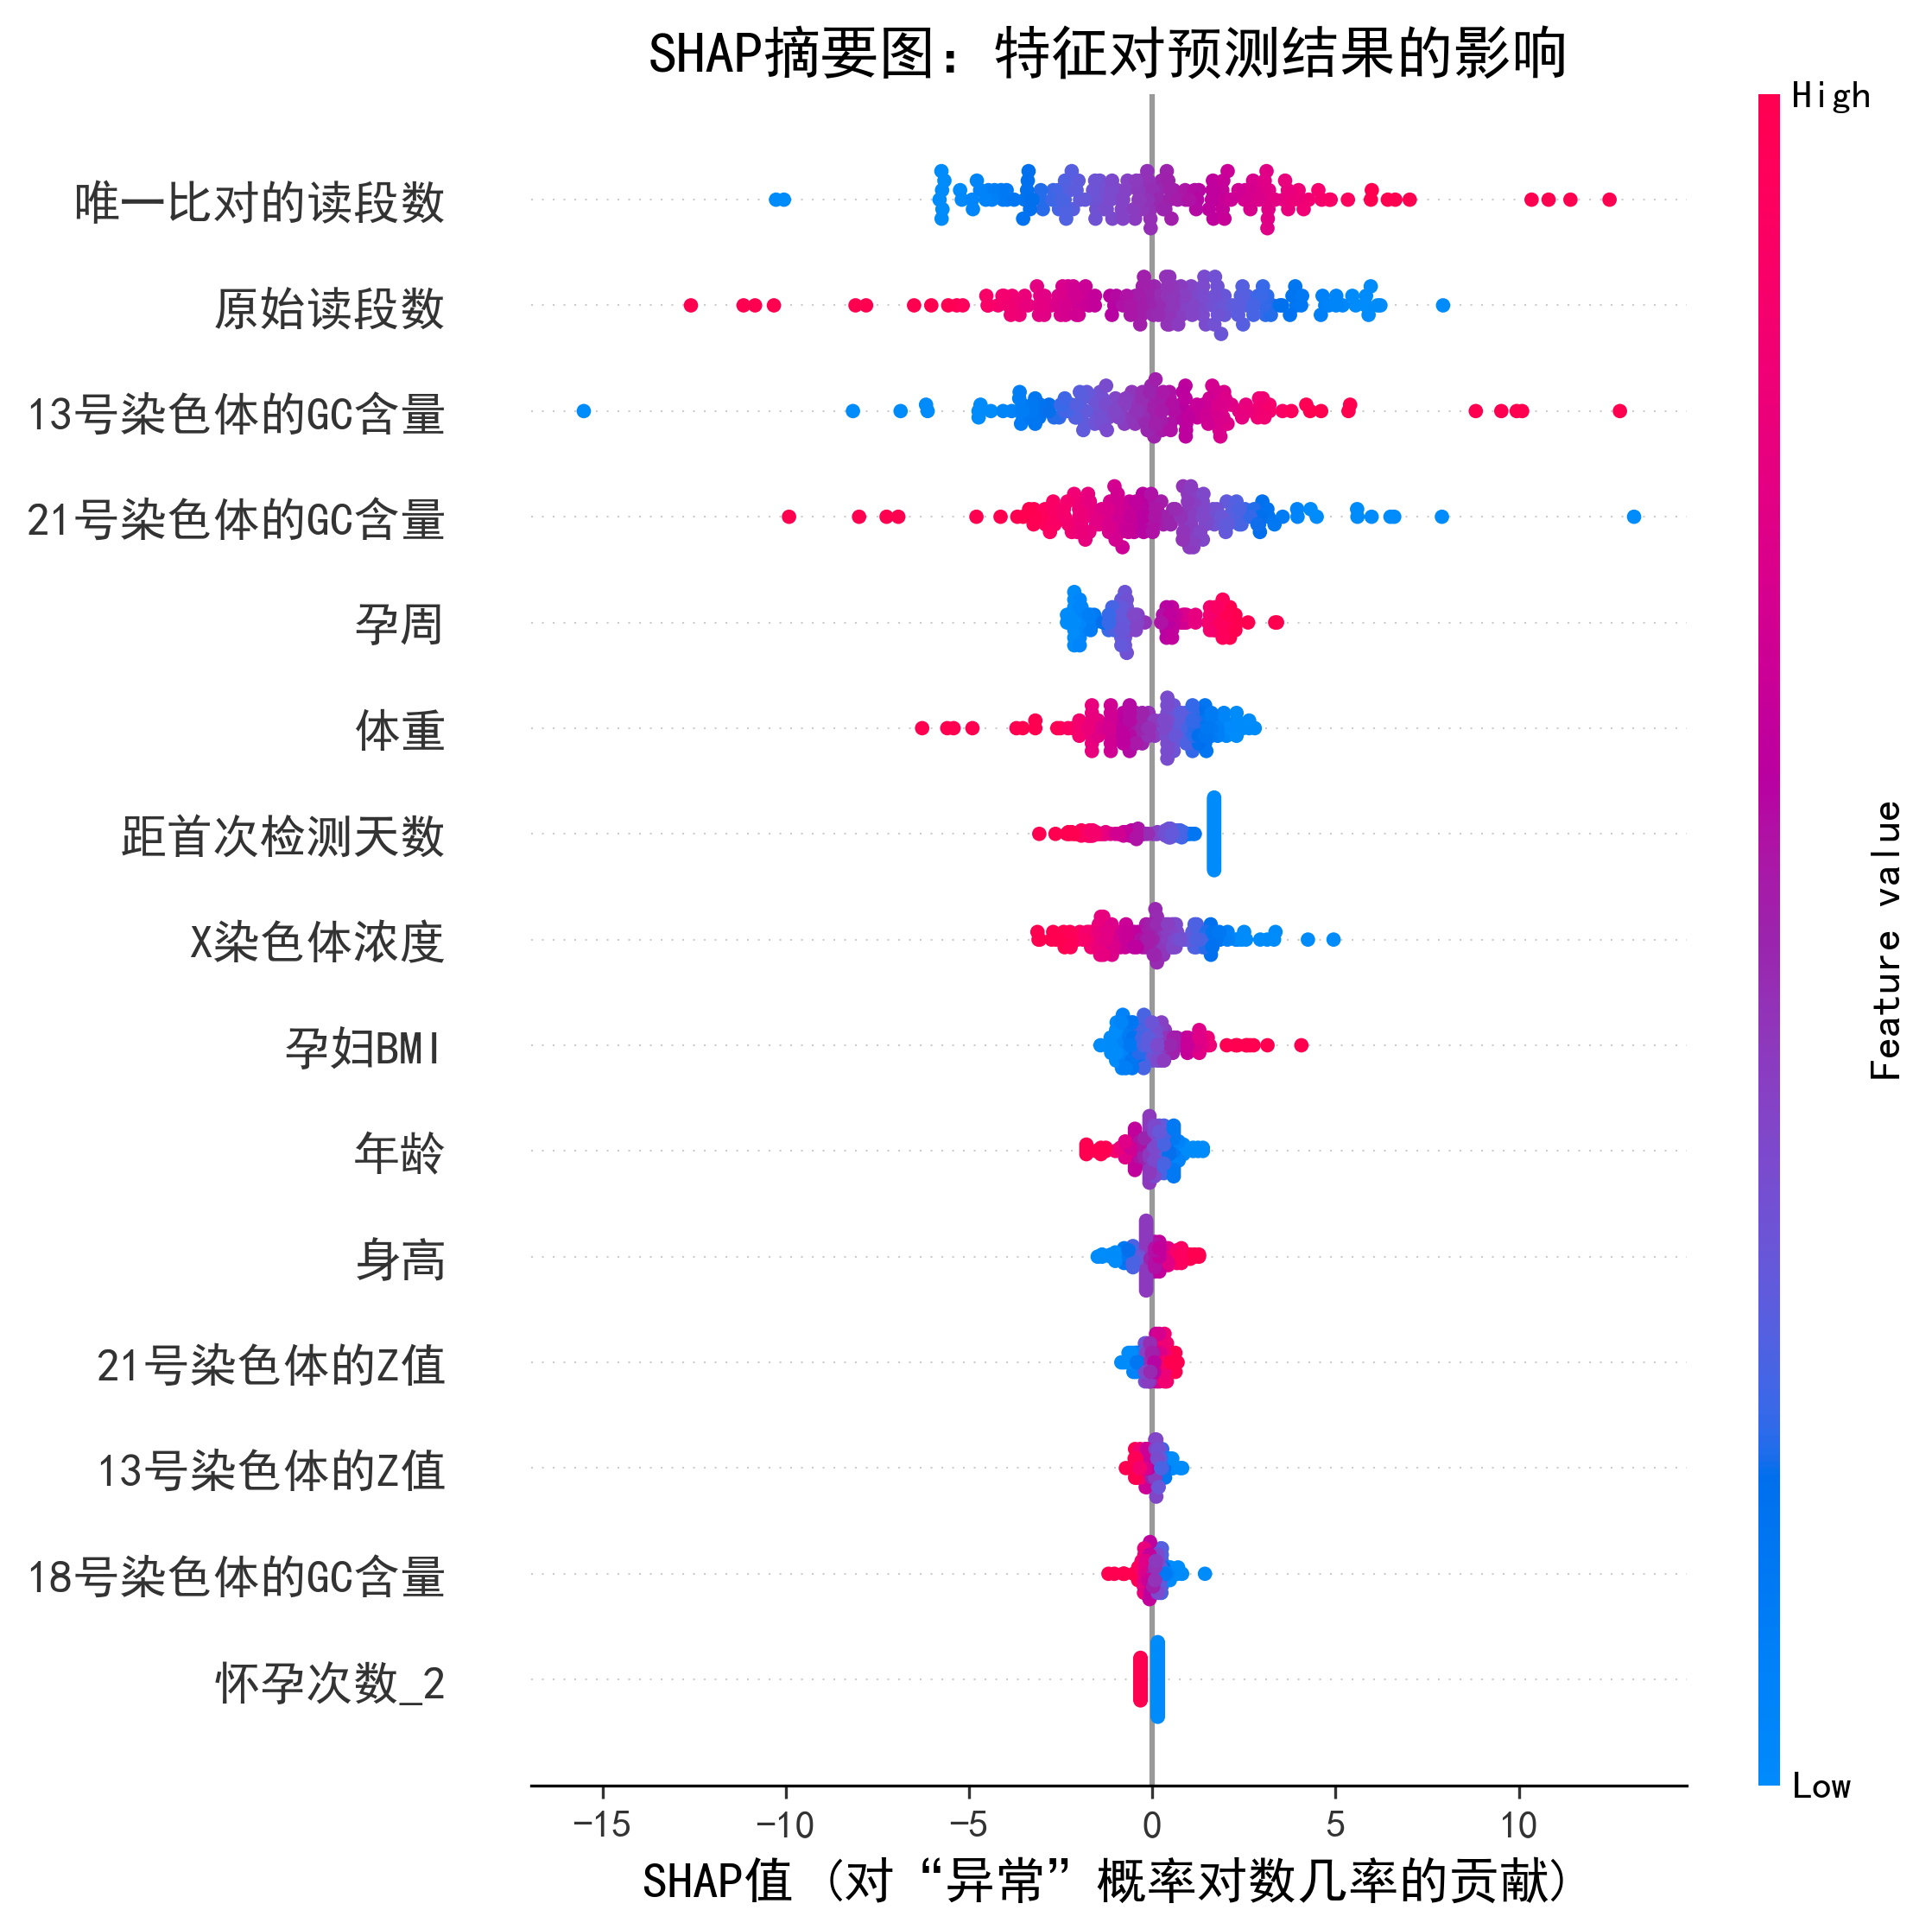
\includegraphics[width=\textwidth]{figs/6问题四/图12_SHAP摘要图.png}
        \caption{SHAP摘要图}
        \label{fig:shap_summary}
    \end{minipage}
\end{figure}

\cref{fig:feature_importance}与\cref{fig:shap_summary}从不同角度展示了模型的决策机制。\cref{fig:feature_importance}呈现了逻辑回归模型为各特征学习到的系数。横轴代表系数的大小，其正负号与数值决定了特征对判定结果为异常概率的影响方向和强度。图中显示，13号染色体的GC含量与唯一比对的读段数具有最大的正向系数，约等于4，表明这些指标数值的增加会使模型判定为异常的可能性显著上升。孕周与孕妇BMI等特征也表现出正向影响。与此相反，原始读段数和21号染色体的GC含量具有较大的负向系数，接近负4，说明这些指标数值的增加会使模型判定为异常的可能性下降。

\cref{fig:shap_summary}则通过SHAP值为模型的决策提供了更细致的个体化解释。图中每一行代表一个特征，按其对模型输出的平均影响大小排序。横轴为SHAP值，每个点代表一个测试样本。点的颜色表示该样本对应特征值的相对高低，红色为高，蓝色为低。该图表明，唯一比对的读段数是对模型预测影响最大的特征，其特征值较高时，SHAP值普遍为正，增加了判定为异常的概率。原始读段数的影响力次之，其特征值较低时，SHAP值倾向于为正。对于临床上关注的指标，例如21号染色体的Z值，图中显示其数值越高，颜色越红，对应的SHAP值也越大，更倾向于将胎儿判定为异常。这一规律与临床诊断21三体综合征的原理相符。

该解释性分析证实，模型的判定主要依据各项染色体Z值、读段数以及GC含量等临床与测序关键指标，其决策逻辑与医学先验知识高度一致，从而验证了模型的有效性与可靠性。


